\chapter{Winning SBIR Contracts}

This lecture is about money before traction: the awkward interval in which a technical invention is real enough to matter, but not yet reduced to a product that customers can buy, test, or even fully understand. Steve Derezinski presents SBIR not as a magic pool of government cash, and not as an exercise in form-filling, but as a particular funding instrument with its own incentives, rules, timing, and failure modes. The lecture belongs in the practical sequence of \emph{Nuts and Bolts of New Ventures}, credited to Joseph Hadzima and MIT OpenCourseWare, with this edition curated by LazyingArt LLC through Video2Book.

\section{Why This Lecture Exists}

The lecture opens with the deliberately attractive phrase ``free government money.'' That is the hook. The subject, however, is narrower and more useful: how to win SBIR awards, not merely how to fill out SBIR forms. Derezinski says that he looked around MIT and found plenty of administrative advice, but not enough practical guidance about the actual winning process. The distinction matters. A form can be complete and still be strategically wrong.

He then establishes his standpoint. He was trained as a mechanical engineer at MIT, worked as a roboticist, patented an algorithm for reducing vibration in the space shuttle robotic arm, went through Sloan, helped build a faculty venture studio at Georgia Tech, and later worked in Kendall Square forming companies from technology. The federal-contract number is stated imprecisely in the transcript: he refers to roughly \(\$40\) million of experience, then to a \(\$23\) million list. The safe reading is simply that he has substantial direct experience as a principal investigator or business lead on federal contracts with agencies including NASA, NSF, DOE, ARPA-E, and DOD.

The first rule follows from that experience:

\begin{equation}
\text{money is not just cash; it is a constraint system.}
\end{equation}

Different money comes with different expectations, different review logic, different time constants, and different consequences if one misuses it. In the lecturer's phrase, money has different ``colors.'' That phrase is not decorative. It is the organizing principle of the chapter.

\section{Disruptive Technology And The Funding Gap}

The first substantive distinction is between incremental and disruptive technology. If the product is incremental, the usual customer-discovery advice works reasonably well. Ask customers what they want, and they will often say: make what I already use cheaper, faster, and better. Their present product gives them the coordinate system in which to answer.

Disruptive technology is different. Customers may not know what to ask for until they can see it, touch it, test it, or imagine using it. This is why the lecture invokes the familiar examples of the faster horse and the product customers cannot describe until it is shown to them. The point is not to romanticize visionaries. The point is operational:

\begin{equation}
\text{disruptive technology}
\quad\Longrightarrow\quad
\text{customer understanding often requires reduction to practice.}
\end{equation}

That creates the funding gap. Universities and government research programs can fund discovery without immediate commercial application. Private capital can fund expansion once a company has customers, traction, and financial history. Between those poles lies the hard interval: the work needed to turn a paper, laboratory result, or prototype into something a market can evaluate.

\subsection{Question \& Answer}

\paragraph{Question.}
If customers cannot yet understand the product, how can a startup validate or fund it?

\paragraph{Answer.}
The lecture's answer is that one should not pretend that ordinary customer traction already exists. The first job is to reduce the technology to practice far enough that customers can respond intelligently. That is precisely where Derezinski places SBIR-type funding: not as a universal best source of startup capital, but as a practical instrument for a deep-technology stage before repeat customer traction.

In symbols, the local problem is

\begin{equation}
\text{paper or lab result}
\;\not\Rightarrow\;
\text{customer-ready product}.
\end{equation}

There is work in between, and the lecture argues that this work is best matched with non-recourse funding.

\section{The Research-To-Market Boundary}

The central slide of the lecture is the research-to-market process. It should be read as a stage map, not as a theorem about all startups. The visible slide gives the sequence

\begin{equation}
\text{Research and inventions}
\rightarrow
\text{Technology Projects}
\rightarrow
\text{Company Projects}
\rightarrow
\text{Funded Company}.
\end{equation}

\begin{figure}
\centering

\includegraphics[width=\linewidth]{lecture_11_figure_02.png}
\caption{Research-to-market funding boundary. The screenshot is the lecture's direct visual evidence for the distinction between technology exploration, customer-focused company execution, and the funding types appropriate on each side of the traction boundary.}
\end{figure}

The two blue boxes are the important ones. A \emph{technology project} is still exploring applications. The technology may have rich research dimensions, but there is not yet a real customer who understands it, has engaged with it, knows how to buy it, or knows how to interact with it. A \emph{company project} comes later: there is a demo, a customer focus, and a need to refine, debug, package, and execute.

Here is a pocket-safe reconstruction of the slide's logic:

\begin{figure}
\centering
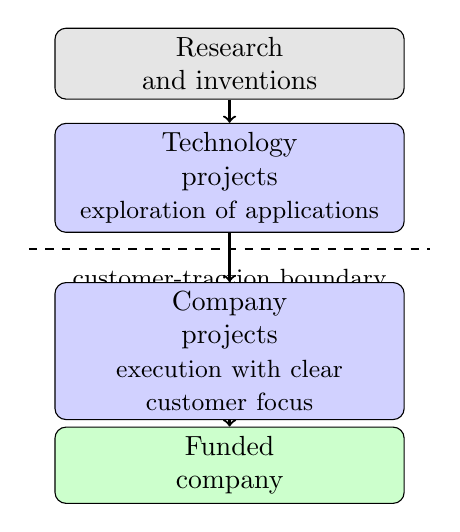
\begin{tikzpicture}[x=1cm,y=1cm]
\node[draw, rounded corners, align=center, text width=4.2cm, minimum height=0.75cm, fill=gray!20] (r) at (0,0)
{Research\\and inventions};

\node[draw, rounded corners, align=center, text width=4.2cm, minimum height=1.05cm, fill=blue!18] (t) at (0,-1.45)
{Technology\\projects\\{\small exploration of applications}};

\draw[dashed, thick] (-2.55,-2.35) -- (2.55,-2.35);
\node[align=center, text width=4.8cm] at (0,-2.75)
{\small customer-traction boundary};

\node[draw, rounded corners, align=center, text width=4.2cm, minimum height=1.05cm, fill=blue!18] (c) at (0,-3.65)
{Company\\projects\\{\small execution with clear customer focus}};

\node[draw, rounded corners, align=center, text width=4.2cm, minimum height=0.75cm, fill=green!20] (f) at (0,-5.10)
{Funded\\company};

\draw[->, thick] (r) -- (t);
\draw[->, thick] (t) -- (c);
\draw[->, thick] (c) -- (f);
\end{tikzpicture}
\caption{A narrow reconstruction of the lecture's research-to-market process for pocket layout.}
\end{figure}

The funding rule is the real payload of the slide:

\begin{align}
\text{no repeat customer traction}
&\Rightarrow
\text{grants and non-recourse funding},\\
\text{repeat customer traction}
&\Rightarrow
\text{equity, debt, VC, angels, or growth capital}.
\end{align}

The warning is strongest on the left side of the boundary. If we take recourse funding while still exploring applications, we create obligations before we know the direction. Derezinski does not say that angels or VCs are bad. He says that the timing is dangerous. On the right side, when customers and traction exist, growth capital can be the right fuel for a pump that is already working.

\section{Incentives: Why SBIR Is Not Venture Capital}

The lecture then quantifies SBIR. The annual federal SBIR pool is described as roughly

\begin{equation}
F_{\text{SBIR}}\approx \$4\text{B per year}.
\end{equation}

Derezinski compares this to a venture-capital fund by using a simple deployment heuristic: venture funds deploy about one fifth of their committed capital per year. If an SBIR-like pool distributes \(\$4\) billion per year, the venture-capital-equivalent fund size is

\begin{align}
F_{\text{VC-equivalent}}
&\approx \frac{\$4\text{B}}{1/5}\\
&\approx \$20\text{B}.
\end{align}

That calculation is not meant to imply that SBIR behaves like venture capital. It is meant to show scale. The behavior is different because the incentives are different.

An angel investor is investing personal money and can decide quickly. A venture capitalist is investing limited partners' money and is pushed toward high return, large equity ownership, and time-sensitive exits. The return pressure can be written schematically as

\begin{equation}
\text{required outcome}
\sim
\text{return as a function of time}.
\end{equation}

If time stretches, the required financial outcome must become much larger. That is why venture capital is a poor fit for many pre-traction technology-exploration projects.

SBIR has another incentive structure. The government does not expect repayment in the ordinary grant sense, and does not require the company to become commercially successful in order for the Phase I work to have been legitimate. The expectation is: do the proposed work, use the funds properly, and report the result. Winning an SBIR may later help private diligence, because external investors may treat it as a signal that technically serious reviewers found the work credible. But the SBIR itself is not venture money.

\subsection{Question \& Answer}

\paragraph{Question.}
What is the first motivation of an SBIR program manager?

\paragraph{Answer.}
The class guesses science, job creation, and proper use of funds. Derezinski accepts those as real motivations, but gives the first motivation as: do not get fired.

That answer explains the bureaucracy. If the proposal is excellent but violates an instruction, the program manager may not be able to repair the defect after submission. The safe administrative move is rejection. Thus the formality is not arbitrary; it follows from the funder's incentive system.

We can summarize the practical ordering as

\begin{enumerate}
\item Do not create a compliance problem for the program manager.
\item Do not embarrass the program manager by appearing careless or unserious.
\item Then make the technical case that the work advances the agency's agenda.
\end{enumerate}

This is why the lecture insists that instructions, eligibility, formatting, and the official solicitation PDF matter. The proposal is not only a technical argument. It is also evidence that the company can be trusted with public funds.

\section{Agencies, Phases, And Program Shape}

The next movement is from incentives to program architecture. SBIR has one name, but not one uniform implementation. The lecturer notes that NSF says SBIR, while DOD speakers may pronounce it as SIBR. The pronunciation is trivial; the underlying point is not. Different agencies implement the program differently.

A useful operational split is between market-driven and mission-driven agencies.

\begin{table}
\centering
\begin{tabular}{p{0.28\linewidth}p{0.30\linewidth}p{0.32\linewidth}}
\hline
Agency type & Where the customer sits & Practical implication\\
\hline
Market-driven & Outside the agency, in the marketplace & The proposal must make a credible case that someone will buy or adopt the technology. NSF and DOE are given as examples.\\
Mission-driven & Inside the agency or its contractor ecosystem & The solicitation may specify a narrow need. DOD and NASA are given as examples.\\
\hline
\end{tabular}
\caption{The lecture's operational distinction between market-driven and mission-driven SBIR agencies.}
\end{table}

Market-driven solicitations may sound broad: do something important in optics, energy, software, or another technology area, and show that the market cares. Mission-driven solicitations may be far more specific: a battery with a particular pack constraint, operating temperature, duration, weight, or field condition. The narrowness is both burden and opportunity. It is harder to match, but it may also reduce the number of serious competitors.

The phase structure gives the next layer of arithmetic:

\begin{align}
p(\text{Phase I win}) &\approx 10\%\text{--}15\%,\\
p(\text{Phase II win}\mid \text{Phase I completed}) &\approx 50\%.
\end{align}

Phase I is the entry point. One must win Phase I to qualify to apply for Phase II. Phase III is commercialization tracking; in the lecturer's framing, there is no ordinary federal Phase III funding. The exception he emphasizes is a Phase IIb-type matching program.

Let \(P\) be qualifying private investment and \(M(P)\) be the federal match. The lecture states a two-to-one private-to-federal match, capped at \(\$500{,}000\). The compact rule is

\begin{equation}
M(P)=\min\left(\frac{P}{2},\$500{,}000\right).
\end{equation}

Two examples make the rule concrete:

\begin{align}
P=\$1{,}000{,}000
&\Rightarrow
M(P)=\$500{,}000,\\
P=\$250{,}000
&\Rightarrow
M(P)=\$125{,}000.
\end{align}

The private investment must be real recourse funding. The lecturer explicitly rejects games such as lending oneself money, collecting the match, and repaying oneself. The required letters and investment structure are there to prove that the private money is genuine.

\section{Eligibility, Multiple Applications, And SBIR Versus STTR}

Eligibility is not only a static checklist. It is a timing problem. The lecture gives the basic constraints:

\begin{align}
\text{employees} &< 500,\\
\text{U.S. citizen or permanent-resident ownership} &\ge 51\%.
\end{align}

The company must be for-profit, and both startups and established companies can apply. Derezinski adds a practical observation from older DOD winner data: one-person companies can win, but the more natural early-company shape is often two to nine people, with some combination of technical and business capability.

The important timing rule is:

\begin{equation}
\text{eligibility is determined at time of award, not merely at submission.}
\end{equation}

That matters for students, postdocs, and founders still inside a university. One may describe a plan to form or join the company by the time of award, but the team, employment, and budget commitments must become true when the award is made. The PI need not necessarily have a PhD or MD, but must have the technical expertise to oversee the scientific and technical work. Derezinski is careful around citizenship and visa questions. The company ownership rule is clear in the lecture; the PI visa details are not turned into a firm legal rule.

\subsection{Question \& Answer}

\paragraph{Question.}
Can we apply to multiple agencies, or does that create a duplicate-award problem?

\paragraph{Answer.}
The distinction is the scope of work. If one proposal funds software development and another funds a different technical component of the same eventual product, those may be distinct scopes. If the same work is copied from NIH to DOD with only the agency name changed, that is the problem.

A useful notation is

\begin{equation}
\operatorname{scope}(P_i)=\text{the work actually funded by proposal }P_i.
\end{equation}

The duplicate-award constraint is

\begin{equation}
\operatorname{scope}(P_i)=\operatorname{scope}(P_j)
\quad\Longrightarrow\quad
\text{do not accept both awards.}
\end{equation}

Different scopes may be disclosed and separately pursued. The same work cannot be funded twice. The lecturer treats this not as a clever optimization problem but as a compliance boundary.

\paragraph{Question.}
Do key team members have to be inside the company?

\paragraph{Answer.}
If a person is named, budgeted, and used as part of the credibility of the proposal, then the company must be able to deliver that person at time of award. Generic later hires are different. A budget line for unspecified software developers is not the same as a named expert whose biography helped the proposal win.

\paragraph{Question.}
How should founders handle incorporation and university conflict of interest?

\paragraph{Answer.}
The lecture deliberately does not give a universal answer. Registration often requires some entity or registration path, but university conflict-of-interest issues depend on the lab, department, institution, and technology rights. The correct note is caution, not invented legal advice.

The SBIR/STTR distinction adds another layer. SBIR permits a research institution partner; STTR requires one. The lecture gives the allocation arithmetic as follows:

\begin{align}
\text{STTR small business share} &\ge 40\%,\\
\text{STTR research institution share} &\ge 30\%.
\end{align}

The minimum required shares sum to

\begin{equation}
40\%+30\%=70\%,
\end{equation}

leaving roughly \(30\%\) of the budget flexible within program and agency constraints. This is one reason STTR can sometimes be strategically useful: more hoops may mean fewer applicants. But the hoops are real, especially when university overhead and conflict-of-interest issues enter.

The overhead example is intentionally rough, but useful. If a \(\$300{,}000\) Phase I award sends \(30\%\) to a university, then

\begin{equation}
0.30\times \$300{,}000=\$90{,}000.
\end{equation}

Derezinski then warns that overhead may reduce the amount available for actual research to something like

\begin{equation}
\$90{,}000
\Rightarrow
\text{roughly }\$45{,}000\text{ or less for the researcher.}
\end{equation}

That is not a formal accounting identity. It is a practical warning: university participation can be valuable when equipment, expertise, or credibility are essential, but it is not free.

\section{Proposal Mechanics, Letters, Quad Charts, And Closing Discipline}

The last movement of the lecture is operational. A proposal is typically about \(25\) pages. For NSF, Derezinski points especially to the project description and letters of support. The project description is described as \(15\) pages and includes an elevator pitch, commercial opportunity, company and team, technical solution, and technical-merit R\&D plan. For Phase I, the center of gravity should remain the technical solution and technical merit.

The review hierarchy is simple:

\begin{equation}
\text{technical merit first}
\quad\text{then}\quad
\text{commercial merit and firm qualifications.}
\end{equation}

A young company may not yet have much firm history. That is why even smaller awards or team accomplishments can matter: they show that a group can act as a cohesive unit rather than as unrelated individuals under a new name.

Letters of support should reduce reviewer uncertainty. A good customer letter says, in effect, that the technology would be valuable if reduced to practice in a particular way. A good investor letter shows serious understanding of both the market opportunity and the technical risk. A good partner letter shows a path toward market access or later investment. Bad letters come from people with weak connection to the technology: paid consultants who obviously benefit from the grant, investors with no technical knowledge, or political supporters with little substantive relevance.

The reviewer has many proposals to read. The easiest answer is no. Thus the proposal should make the yes easy:

\begin{equation}
\text{review burden high}
\quad\Rightarrow\quad
\text{make credibility visible inside the proposal itself.}
\end{equation}

The lecture then turns to the quad chart or project pitch. This is the recommended first outreach instrument. Before spending too much money on company formation or administrative machinery, prepare a compact description of the technology, objectives, market opportunity, and team. NSF has a project-pitch process; other agencies commonly respond to a quad chart. Derezinski calls the quad chart a kind of love language for the SBIR community because it packages the opportunity in a format program managers can digest.

The workflow is sequential:

\begin{enumerate}
\item Identify agencies and topics that could fund the technology.
\item Look for previously funded awards similar to the project.
\item Find the official solicitation PDF and the relevant program contact.
\item Prepare the quad chart or project pitch.
\item Ask the program manager for fit feedback, not unfair proposal coaching.
\item Ask who else should be consulted.
\item Then proceed with registration, company administration, and full proposal work.
\end{enumerate}

The timing arithmetic is also part of the discipline:

\begin{align}
T_{\text{broad proposal}} &\approx 2\text{ months},\\
T_{\text{specific mission fit}} &\approx T_{\text{broad proposal}}+1\text{ month},\\
T_{\text{registrations}} &\approx 30\text{ days}.
\end{align}

Registrations can run in parallel with proposal writing, but they should not be ignored. The official solicitation PDF is the ground truth. Consultants, summaries, templates, and advice may help, but the legal and procedural authority is the solicitation itself. If the solicitation does not answer the question, ask the program manager.

Two final cautions close the lecture. First, AI can help draft. Derezinski's rough grading metaphor is

\begin{equation}
\text{AI}: F\to B,
\qquad
\text{human judgment}: B\to A/A^+.
\end{equation}

That is, AI may improve a bad draft into a serviceable draft, but funded proposals still require human judgment, technical specificity, relationship-building, and real credibility. People fund people.

Second, diligence increases as the money increases. For Phase II, the company may need to show an accounting system, timecards, proper allocation of labor, proof, and sign-off. The transcript's audit acronym is uncertain, but the operational requirement is not:

\begin{equation}
\text{government money}
\Rightarrow
\text{allocation evidence, time records, accounting control, and sign-off.}
\end{equation}

Fast-track applications receive a similar caution. They can be appropriate when commercial partners are already lined up and the solicitation fit is unusually strong. But because many applicants want to skip directly toward the larger money, competition can be tougher. This is exactly the sort of decision that should be discussed with the program manager.

\section{Summary}

The lecture begins with the promise of free government money and ends with homework. That arc is the point. SBIR is not free in the sense of effortless; it is non-recourse funding with rules, deadlines, incentives, and compliance obligations.

The central map is the customer-traction boundary. Before repeat customer traction, a deep-technology company may need grants or non-recourse funding to reduce the invention to practice. After repeat traction, recourse capital can become appropriate growth fuel. SBIR sits in the gap, but each agency implements it differently, and each solicitation must be treated as its own ground truth.

The practical prescription is therefore disciplined rather than glamorous: understand the agency, understand the phase, disclose related applications, avoid duplicate scopes of work, be careful with university partners, write for technical merit, use meaningful letters of support, prepare the quad chart, speak to the right program manager, and treat a fast no as useful information.